\documentclass[aps,prl,twocolumn,superscriptaddress]{revtex4-2}
\usepackage{physics}
\usepackage{amsmath}
\usepackage{graphicx}
\usepackage{dsfont}
\usepackage{mathrsfs}
\usepackage{braket}

\begin{document}
\title{Entanglement Dynamics in a Driven Spin Chain}
\author{L. Wei}
\affiliation{Institute of Physics, Example University}
\author{R. Patel}
\affiliation{Department of Physics, Other University}
\email{rpatel@example.edu}
\date{\today}

\begin{abstract}
We study the time evolution of entanglement entropy in a periodically driven XXZ chain.
\end{abstract}
\pacs{03.67.Mn, 05.30.-d}
\keywords{entanglement, Floquet, spin chains}
\maketitle

\section{Model}
The Hamiltonian is
\begin{equation}
  \hat H = -J \sum_{i} \qty( \sigma^x_i \sigma^x_{i+1} + \Delta\, \sigma^z_i \sigma^z_{i+1} ) + h(t) \sum_i \sigma^z_i .
  \label{eq:ham}
\end{equation}
The Schr\"odinger equation reads $i\hbar \dv{t}\ket{\psi(t)} = \hat H \ket{\psi(t)}$, and the expectation
$\expval{\hat O}{\psi} = \mel{\psi}{\hat O}{\psi}$. The commutator $\comm{\hat x}{\hat p} = i\hbar \mathds{1}$.
The partial derivative $\pdv{f}{x}{y}$ and $\pdv[2]{f}{x}$ appear in the continuum limit.

The density matrix $\rho = \dyad{\psi}$ has $\Tr \rho = 1$, and we write $\mathscr{H}$ for the Hilbert space.
With the braket package: $\Braket{\phi | \hat A | \psi}$ and $\Set{x | x > 0}$.

\begin{equation}
  S_A = -\tr\qty(\rho_A \log \rho_A), \qquad \abs{\vb{r}} = \norm{\vb{r}}, \qquad \grad \cdot \vb{E} = \rho/\varepsilon_0 .
\end{equation}

The matrix $\mqty(a & b \\ c & d)$ and $\pmqty{1 & 0 \\ 0 & -1}$ and $\order{\epsilon^2}$.

\section{Results}
Figure~\ref{fig:ent} shows linear growth followed by saturation~\cite{smith2020}.
\begin{figure}[t]
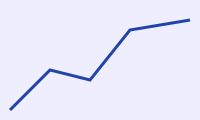
\includegraphics[width=\columnwidth]{plot.svg}
\caption{Entanglement entropy versus time for $L = 20$.}
\label{fig:ent}
\end{figure}

\begin{acknowledgments}
We thank the funding agency.
\end{acknowledgments}

\bibliography{refs}
\end{document}
